\documentclass[svgnames,11pt]{beamer}
\setbeamercolor{structure}{fg=SlateGray}
\usetheme{Goettingen}
\input{/home/tof/Documents/Cozy/latex-include/preambule_commun.tex}
\author[]{Christophe Viroulaud}
\title{Suite de Fibonacci}
\date{}
%\logo{}
%\institute{Seconde SNT}
%\institute{Première NSI}
\institute{Terminale NSI}
\setbeamertemplate{navigation symbols}{}
\setbeamertemplate{footline}[frame number]
\usepackage{tikz}

\begin{document}
\begin{frame}
    \titlepage
\end{frame}

\section{Problématique}
\begin{frame}
    \frametitle{}
    $$
        F_n = \left\{
        \begin{array}{ll}
            F_0 = 0                 & \mbox{si } n=0 \\
            F_1=1                   & \mbox{si } n=1 \\
            F_{n} = F_{n-1}+F_{n-2} & \mbox{si } n>1 \\
        \end{array}
        \right.
    $$
    \begin{center}
        \framebox{Comment obtenir un calcul efficace des termes de la suite?}
    \end{center}
\end{frame}

\section{Mise en évidence du problème}
\begin{frame}
    \frametitle{}
    \lstinputlisting[firstline=9 ,lastline= 19]{"scripts/fibo.py"}

\end{frame}

\begin{frame}
    \frametitle{}
    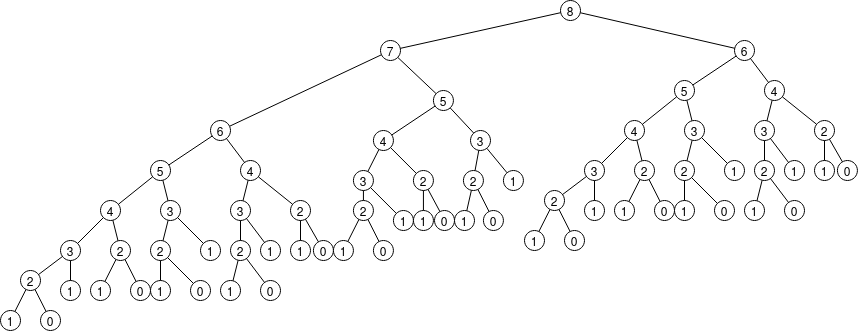
\includegraphics[width=\textwidth,height=8cm]{ressources/fibo1.png}

\end{frame}

\begin{frame}
    \frametitle{}

    \begin{activite}
        \begin{enumerate}
            \item Tester la fonction \emph{fibo} pour $n=8$, $n=10$.
            \item À l'aide d'une variable globale (c'est mal) \emph{compteur}, observer le nombre d'appels réalisés en fonction de \emph{n}.
        \end{enumerate}
    \end{activite}

\end{frame}

\begin{frame}
    \frametitle{}
    \lstinputlisting[firstline=21 ,lastline= 34]{"scripts/fibo.py"}

\end{frame}
\begin{frame}
    \frametitle{Nombre d'appels en fonction de n}
    \begin{center}
        \centering
        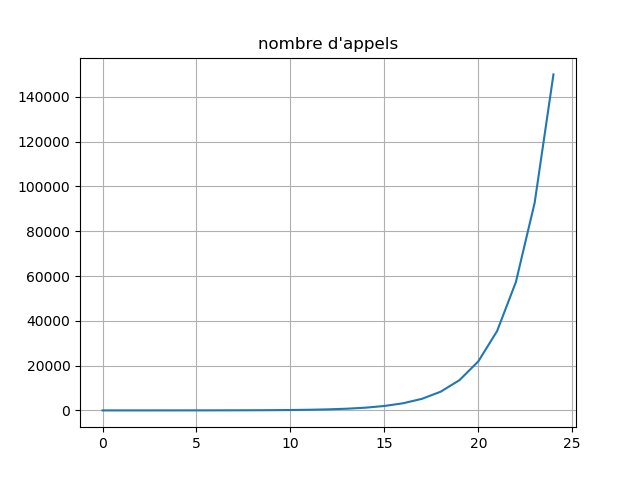
\includegraphics[width=10cm]{ressources/nb-appels.png}
        \label{IMG}
    \end{center}
\end{frame}

\section{Programmation dynamique}
\subsection{Approche top-down}
\begin{frame}
    \frametitle{}

    Une amélioration de l'approche \emph{diviser pour régner}

\end{frame}
\begin{frame}
    \frametitle{}

    \lstinputlisting[firstline=9 ,lastline= 24,basicstyle=\small]{"scripts/fibo-dyn.py"}

\end{frame}
\begin{frame}
    \frametitle{Appel de la fonction}
    \lstinputlisting[firstline=26 ,lastline= 28]{"scripts/fibo-dyn.py"}
\end{frame}
\begin{frame}
    \frametitle{}

    \begin{aretenir}[]
        La \emph{mémoïsation} consiste à la \emph{mise en cache} les valeurs déjà calculées pour pouvoir être réutilisées.
    \end{aretenir}

\end{frame}

\begin{frame}
    \frametitle{}

    \begin{activite}
        Tester la fonction en approche top-down. Compter le nombre d'appels.
    \end{activite}

\end{frame}
\begin{frame}
    \frametitle{Nombre d'appels en fonction de n}

    \begin{center}
        \centering
        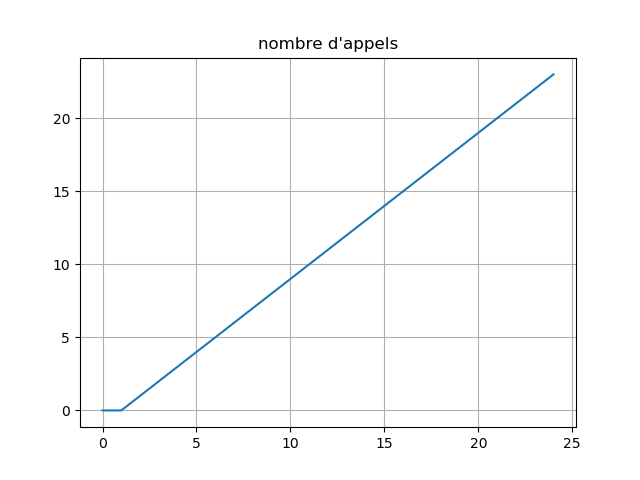
\includegraphics[width=10cm]{ressources/nb-appels-dyn.png}
        \label{IMG}
    \end{center}

\end{frame}

\begin{frame}
    \frametitle{}

    \begin{center}
        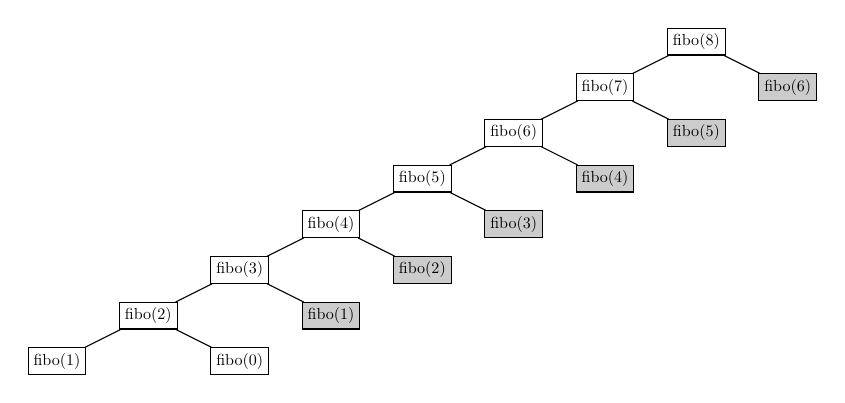
\begin{tikzpicture}[scale=0.58, transform shape]
            \node[draw] (A) at (0,0) {fibo(8)};
            \node[draw] (B) at (-2,-1) {fibo(7)};
            \node[draw,fill=gray!40] (C) at (2,-1) {fibo(6)};
            \node[draw] (D) at (-4,-2) {fibo(6)};
            \node[draw,fill=gray!40] (E) at (0,-2) {fibo(5)};
            \node[draw] (F) at (-6,-3) {fibo(5)};
            \node[draw,fill=gray!40] (H) at (-2,-3) {fibo(4)};
            \node[draw] (I) at (-8,-4) {fibo(4)};
            \node[draw,fill=gray!40] (J) at (-4,-4) {fibo(3)};
            \node[draw] (K) at (-10,-5) {fibo(3)};
            \node[draw,fill=gray!40] (M) at (-6,-5) {fibo(2)};
            \node[draw] (O) at (-12,-6) {fibo(2)};
            \node[draw,fill=gray!40] (P) at (-8,-6) {fibo(1)};
            \node[draw] (Q) at (-14,-7) {fibo(1)};
            \node[draw] (R) at (-10,-7) {fibo(0)};

            \draw (A) -- (B);
            \draw (A) -- (C);
            \draw (B) -- (D);
            \draw (B) -- (E);
            \draw (D) -- (F);
            \draw (D) -- (H);
            \draw (F) -- (I);
            \draw (F) -- (J);
            \draw (I) -- (K);
            \draw (I) -- (M);
            \draw (K) -- (O);
            \draw (K) -- (P);
            \draw (O) -- (Q);
            \draw (O) -- (R);
        \end{tikzpicture}
        \captionof{figure}{Appels récursifs pour $n=8$}
        \label{moncode}
    \end{center}

\end{frame}

\subsection{Bottom-up}
\begin{frame}
    \frametitle{}

    Approche \emph{itérative} qui résout d'abord les sous-problèmes.

\end{frame}

\begin{frame}
    \frametitle{}

    \begin{center}
        \lstinputlisting[firstline=30 ,lastline= 35,basicstyle=\small]{"scripts/fibo-dyn.py"}
        \captionof{code}{Approche bottom-up}
        \label{moncode}
    \end{center}

\end{frame}
\begin{frame}
    \frametitle{}

    \begin{activite}
        Combien d'itérations effectue-t-on?
    \end{activite}

\end{frame}

\begin{frame}
    \frametitle{Top-down ou Bottom-up?}

    \begin{itemize}
        \item<1-> Complexité en temps souvent équivalente,
        \item<2-> Complexité en espace peut être optimisée: s'il est simple de déterminer quels résultats vont être nécessaires, l'approche bottom-up est intéressante.
    \end{itemize}

\end{frame}

\begin{frame}
    \frametitle{Approche bottom-up optimisée en espace}

    \lstinputlisting[firstline=39 ,lastline= 44,basicstyle=\small]{"scripts/fibo-dyn.py"}

\end{frame}
\end{document}